


 Suppose a circle has a $60^\circ$ arc removed.  Then, the endpoints of the remaining arc are connected with a line segment to create the following shape:

\begin{center}
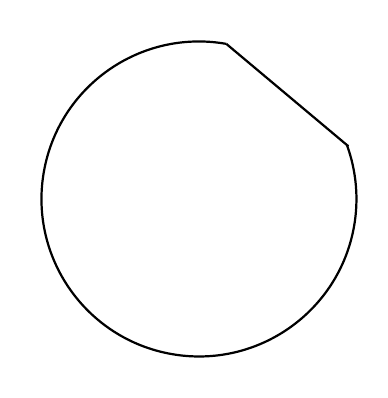
\begin{tikzpicture}
    \draw[thick] (0,2) arc (80:380:2);
   
    \draw[thick] (1.55,.7)--(0,2);
         
      
       
               
\end{tikzpicture} 
\end{center}
If the original circle had a radius of 6, then what is the perimeter of this shape?



\ifsat
	\begin{enumerate}[label=\Alph*)]
		\item  $10 \pi$ 
		\item  $10\pi+6$ % 
		\item  $12\pi+6$
		\item  $12\pi+12$
	\end{enumerate}
\else
\fi

\ifacteven
	\begin{enumerate}[label=\textbf{\Alph*.},itemsep=\fill,align=left]
		\setcounter{enumii}{5}
		\item  $10 \pi$ 
		\item  $10\pi+6$ % 
		\item  $12\pi$ 
		\addtocounter{enumii}{1}
		\item  $12\pi+6$
		\item  $12\pi+12$
	\end{enumerate}
\else
\fi

\ifactodd
	\begin{enumerate}[label=\textbf{\Alph*.},itemsep=\fill,align=left]
		\item  $10 \pi$ 
		\item  $10\pi+6$ % 
		\item  $12\pi$ 
		\item  $12\pi+6$
		\item  $12\pi+12$
	\end{enumerate}
\else
\fi

\ifgridin
  $10\pi+6$ % 
		
\else
\fi

